\documentclass[a4paper,12pt,twocolumn]{report}
\usepackage[utf8]{inputenc}
\usepackage{graphicx}
\usepackage{natbib}   % omit 'round' option if you prefer square brackets
\usepackage{hyperref}
\graphicspath{ {img/} }


% Title Page
\title{CM30229 - Circumnavigation using Lejos}
\author{Dominic Hauton}


\begin{document}
\maketitle
\bibliographystyle{plainnat}

\section{Introduction}
% All of your courseworks are designed primarily to give you experience in developing intelligent control and/or cognitive systems. However, the course is also intended to give you experience and feedback in writing about research. To this end, you will be writing research reports of about two pages, using exactly this format.

% The Introduction of a research report should give a brief description of what you you tried to do (your hypothesis), and the outcome. It should also give some idea about why you have done it (motivation). In doing this, you may also give a brief background argument. I expect you to cite a paper or two for this motivational context. For coursework 1, one of the papers you should probably cite is Brooks (1991), since you have been asked to take a fairly reactive approach to developing robot intelligence.

% Coursework one requires you to construct a robot capable of circumnavigating rooms or other closed spaces (don’t worry about doorways – just close or block them.) Ideally this should work in “natural” (unaltered) indoor environments with a variety of obstacles along the walls, but often people build up some barriers. However, the report should not be about the entire experience of building a robot, but rather it should present a single hypothesis you tested on your completed robot about how to improve its intelligence.

The goal of this research is to see the effect of changing the rate of sensing on the navigation capabilities of a rover. The rover is built using parts from the LEGO Mindstorm NXJ kit. Four sensors are utilised for sensing; a \emph{Sonar}, \emph{Light Sensor} and \emph{Bump Sensor} (x2), and three motors provide movement.

The sonar is mounted on a pivot to allow for measurements in multiple directions, as shown in figure \ref{fig:stanley-head}. Two driven wheels are used for drive and a trolley wheel is placed at the back for stability.

\begin{figure}[b]
 \includegraphics[width=0.5\textwidth]{headshot}
 \caption{Rover Head Sensor}
 \label{fig:stanley-head}
\end{figure}

During development a reactive approach is taken, using the subsumption architecture \citep{wooldridge2009introduction} to allow the rover to determine its current situation.

The use of the subsumption architecture is based on \cite{brooks1991intelligence}' thesis that Intelligence is an emergent property of certain complex systems. During development this subsumption approach is added into the perception mechanism.

\section{Approach}

% The approach describes in detail exactly what you have done. This section is longer, and should ideally include some experiments you set up, for example to determine in what conditions you could get better results from the robot. The approach should be in sufficient detail that another person could replicate your experiments. You may cite other papers here too if you are taking an approach from another paper, or modifying it only slightly.

% Please do mention who shared your robot in the approach section, and the extent to which you worked together. The objective here is to learn. How much you work together is totally up to you so long as you each write your report independently.

% Submissions should be in PDF or HTML, preferably derived from this latex format, certainly in 12 point font. I recommend making HTML by using latex plus htlatex, but you can construct your report using any tool you please. Note that this specification is exactly 2 pages long, so an HTML report should be no longer than this. Figures (both drawn plans and photos) are encouraged for marks and clarity and do not count either for or against page length. The 1–2 pages are counting text only (not citations). But remember, don’t spend too much time on this coursework! You should spend about 19 hours total on each coursework, about 4 of which will be writing up. The coursework should be uploaded to Moodle by 11pm on Friday 3 March at the latest, but feel free to submit it (much) sooner.

% To quantify the outcomes of this coursework, you may want to think about questions such as contrasting the addition of extra control algorithms, changing the physical shape of the robot, or trying different target sonar readings for maintaining a particular distance from the wall in a variety of contexts. These can be quantified in terms of the circuit time for the robot, the success rate, or any other metric you can think of.

% For coursework one, it is quite likely that you will not have initially thought of a hypothesis to test, but will rather just have tried to make the robot work. However, in your exploration (both with the robot and with your reading) you should always be looking to something that seems to make a difference in performance, and then try to capture what that something is. Can you describe it ex you get given how much change you make to some parameter on the robot? Don’t forget to consider things such as the battery charge, operating in daylight, or proximity to other sonar-using robots as possible explanations for strange behaviour.

The initial design of the rover is a simple reflex agent as described by \cite{russell1995modern}. This takes numerical sensor readings, and uses transduction converting them to a qualitative proximity label in every cardinal direction, making immediate decisions based on these readings. This allows the rover to react to a crash but gives no context for recovery.

The final design uses \cite{russell1995modern}'s model-based reflex agent. This allows the sensors to modify the state at individual rates. There are two sensing thread loops as shown in figure \ref{fig:perception}. This is done to prevent the sonar slowing down other sensors.

As the front sensor uses three\footnote{Bump, light and sonar sensor} separate sensors for proximity detection the closest, most important, result is taken. To improve sensor quality 15 readings are taken every measurement and any reading more than two standard deviations away from the mean is thrown out. The remainder of the readings are averaged.

To account for arena variances, a calibration routine is used. This requests several rover placements a given distance from the arena wall on each side.

\begin{figure}
 \includegraphics[width=0.5\textwidth]{sensing-diagram}
 \caption{Final Perception Architecture}
 \label{fig:perception}
\end{figure}

A decision loop reads the state and determines a meta-state\footnote{Such as \emph{TOO\_CLOSE\_TO\_WALL} or \emph{WALL\_NOT\_FOUND}.} from the current state using a subsumption architecture. If the rover is \emph{NEAR} something to the front, it has crashed and it does not matter that it is \emph{NEAR} an object on the side too. This meta-state is then used in the action planner, which selects the best action given a meta-state. If the rover is crashed and it is \emph{NEAR} an object to the left, it does not try to reverse to the left.

The meta-state also directs the sonar. If it is following a wall on the left and has found the wall, it skips the reading on the right as it is irrelevant to the navigation. This system describes the platform for experimentation. The goal is to find if there is an optimal sensing rate.

The rover is run at a tick rate (measurements per second) of 5, 25 and 45. During a run the rover performs 10 laps of the test track (fig. \ref{fig:area}), and the number of bump sensor activations was recorded programmatically.

Each run is done twice. The hypothesis is that the rover will perform better with a higher tick rate, but with diminishing returns. If the rover is stuck in a corner, the experiment is restarted. During each run, the rover is started in the bottom left hand corner of the arena (fig. \ref{fig:area}) facing the left wall. The experiment is conducted with a variety of obstacle types and sizes to produce a generalised result.

\begin{figure}[t]
 \includegraphics[width=0.5\textwidth]{test-area-layout}
 \caption{Test Area Layout}
 \label{fig:area}
\end{figure}

The rover was shared with Ryan Cullen. Dominic Hauton built the rover itself, optimising it's design and creating the perception system in the code, which continuously modifies proximity readings in the state, indicating how close the rover is to an object in all four cardinal directions. At this point Ryan forked the code and action selection is developed individually.

\begin{figure}
 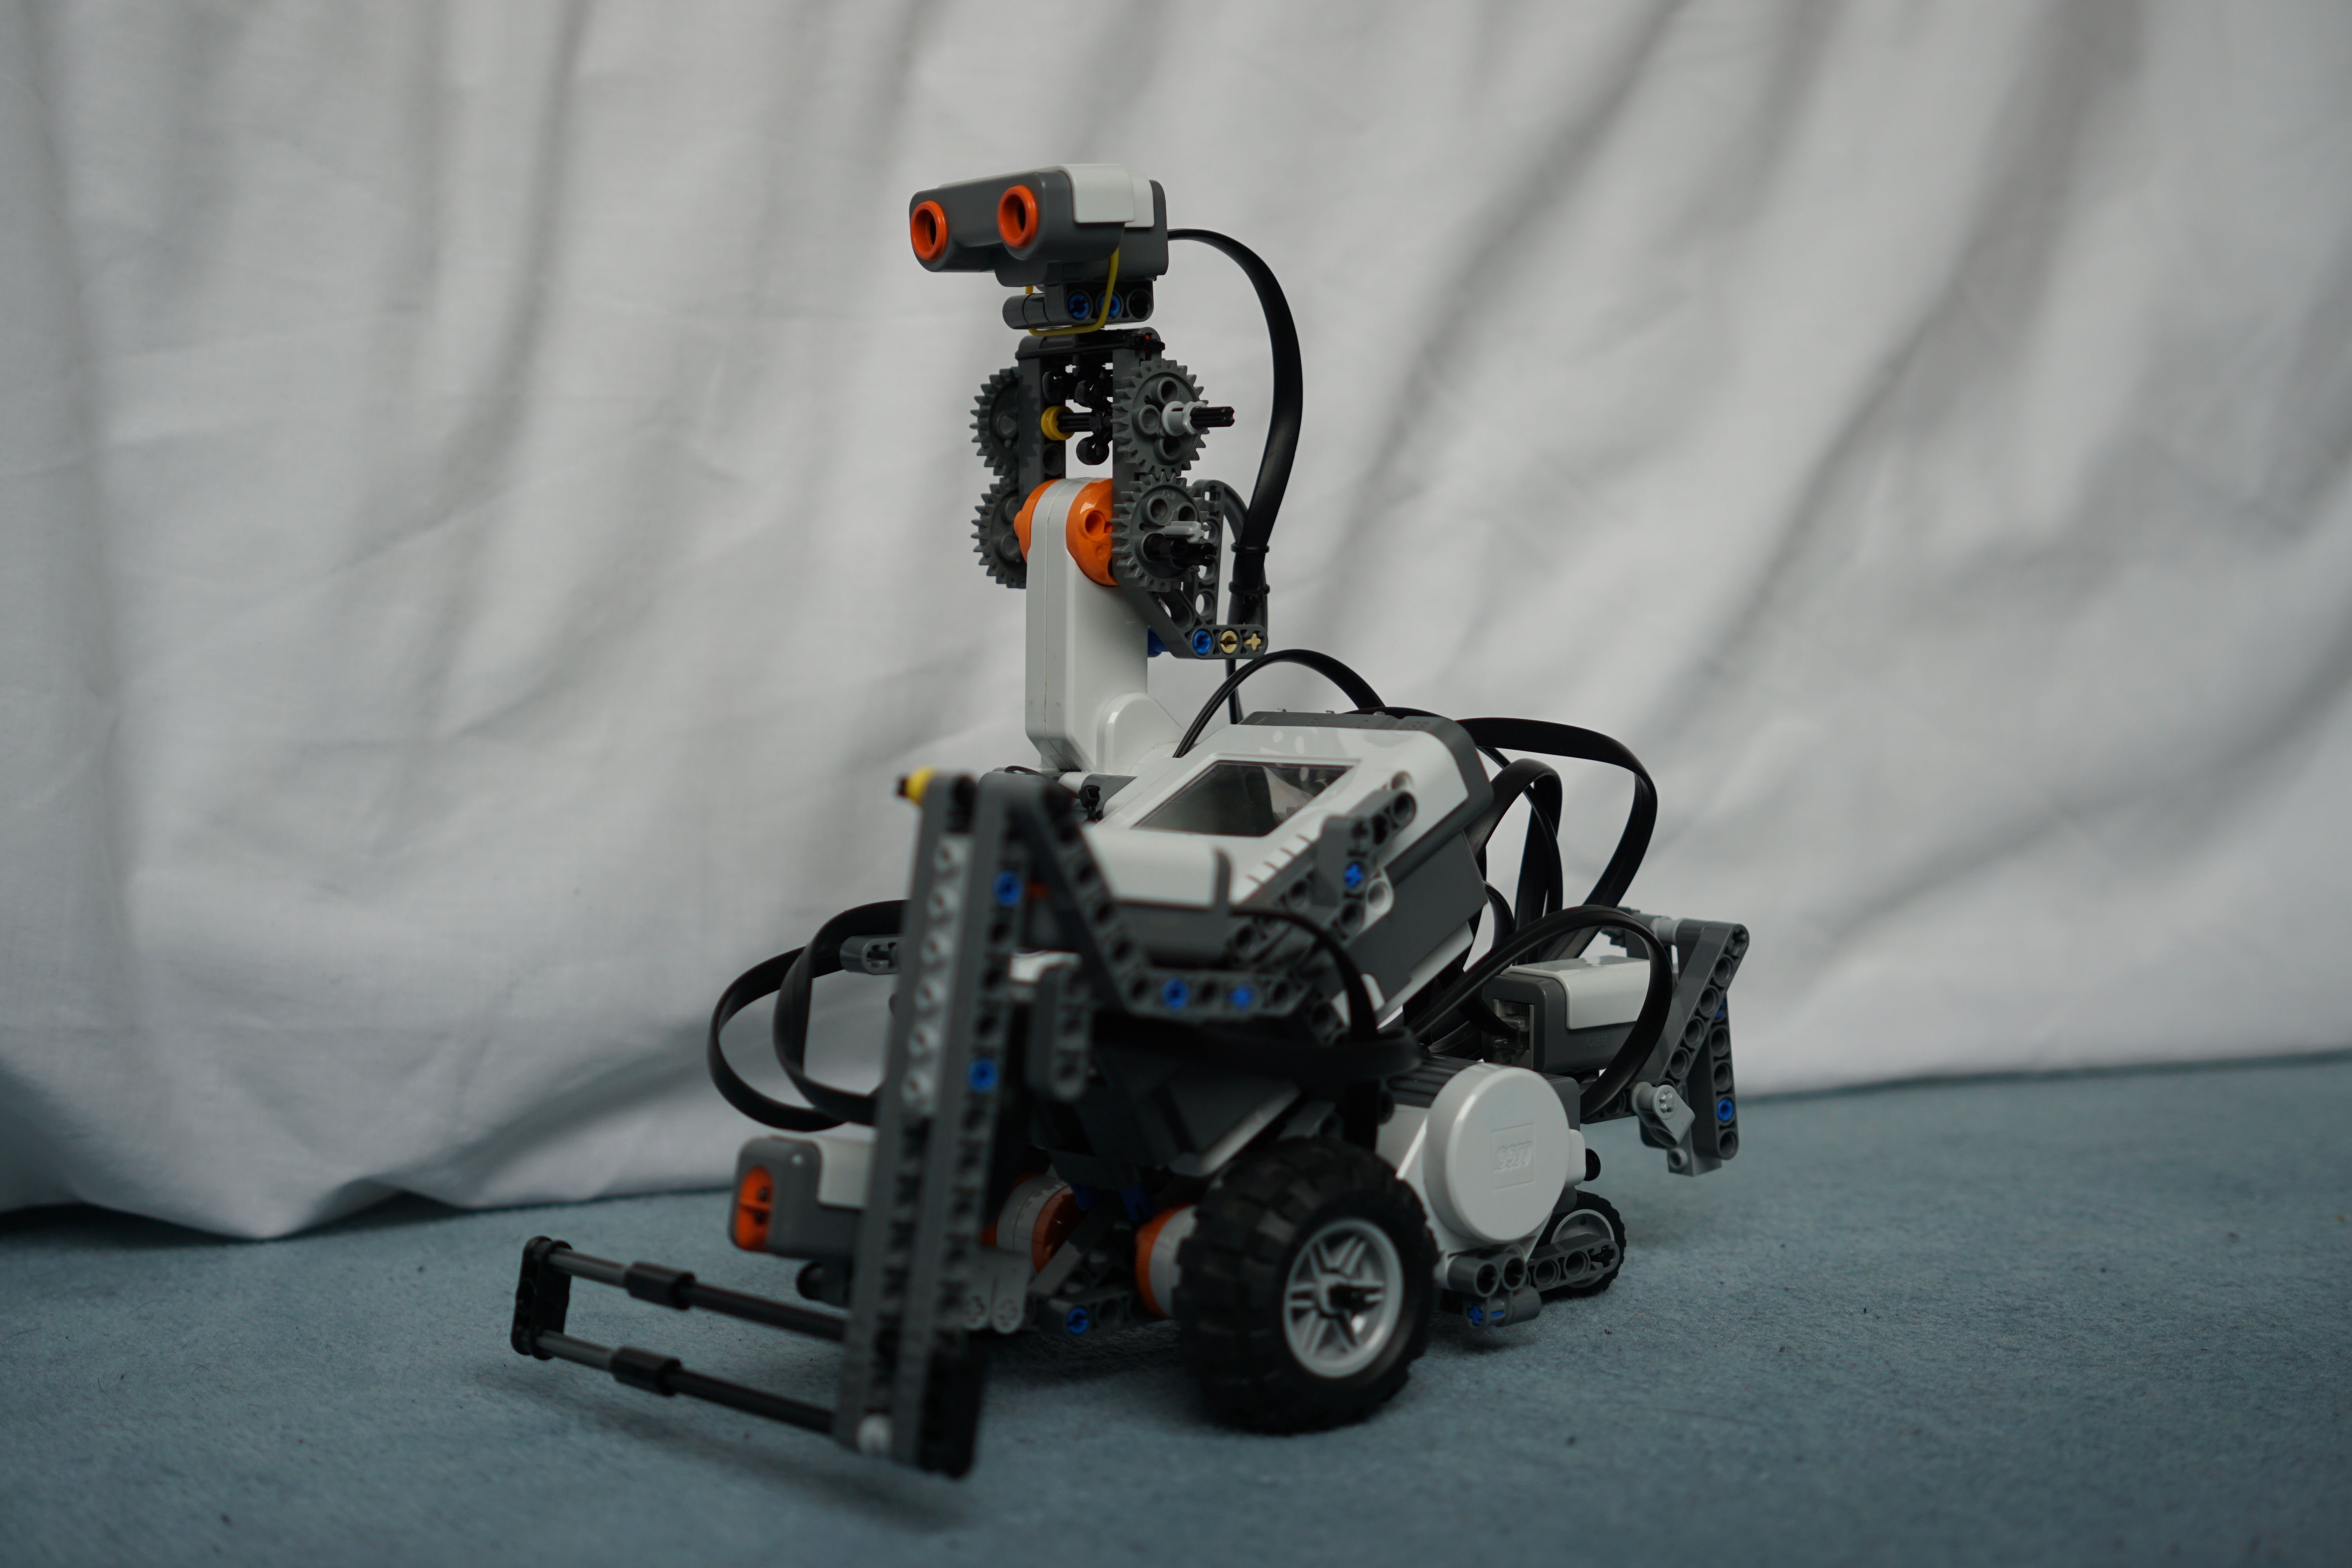
\includegraphics[width=0.5\textwidth]{full}
 \caption{Stanley Rover}
 \label{fig:stanley}
\end{figure}

\section{Results}

% The results section describes the outcomes. This should be purely factual descriptions, including qualitative outcomes, quantitative outcomes and possibly statistics. For example, you could report the average speed around a circuit in two conditions plus standard deviations and a significance test to tell whether you have evidence that the conditions lead to different results. For coursework 1, this must include video. Typically, the results section can be surprisingly short, since the Approach section is the one giving details. Results are purely and only factual outcomes (no alternative facts).

% With respect to your personal results, if you describe a reasonably-well working system in a comprehensible manner you will pass. If you competently fill in all of these sections as described in this specification, you will get at least 55. Getting a mark over 70 requires demonstrating insight, creativity and / or understanding that goes beyond the basics laid out for you in this document. For example, an insightful comment about one or more cited papers supported by evidence from your experience might get you these extra marks. So might a particularly accurate and replicable account of your approach and results.

The results of the experiment are consistent with the hypothesis. With this positive result the experiment is also conducted after doubling the rover movement speed. A higher tick rate is found to help the rover at higher speeds, leading to the conclusion that the faster the rover moves, the faster it needs to sense the environment around it.

As the results for one lap are inconsistent, the rover performs two runs of 10 laps. Both 10 lap runs were within 2 bumps per lap of each other on average, which was within the required 0.10 p-value for statistical significance.

\begin{table}
\centering
\caption{Bumps per lap at two speeds}
\label{my-label}
\begin{tabular}{|l|c|c|c|}
\hline
Tickrate         & 5  & 25 & 45 \\ \hline
Slow & 23 \pm 2 & 14 \pm 0 & 16 \pm 1 \\ \hline
Fast & 53 \pm 3 & 46 \pm 2 & 26 \pm 2 \\ \hline
\end{tabular}
\end{table}

The video found at \url{https://youtu.be/LOPdO0w1Uec} depicts the start of a trail run.

\section{Discussion}

% The discussion is the most discursive part of your paper, it may include speculation. You should discuss the extent to which your results addressed the questions described in your introduction, and what the results imply about your own work and AI or robotics more broadly. You might suggest other experimental protocols that could have given different results and lessons learned. This can be a longer section, and may again include citations if you compare or contrast to other published accounts.

The results closely match the hypothesis, however, the sensing speed of the sonar, which is the key part of the navigation logic, is limited due to physical speed. A second sonar that does not require physical movement for sensing may improve the navigation of the rover.

Although the arena environment was kept as consistent as possible, the light sensor is very susceptible to bright light and occasionally reacted to the room light being in front of it. To make sonar readings consistent the arena is covered with hard surfaces, but even with the arena, materials of different hardness result in different distance readings.

The main take away from the research, is that to improve navigation of a rover; sensing should be increased as far as they add a tangible benefit to navigation, and the faster the movement the more important this is. In applications such as quadcopters loop times affect flight characteristics, but enabling faster loop times might mean disabling other features so this left adjustable in drone software for users. \citep{betaflight}. It is important for these users to understand the significance of this sensing rate change.

\section{Conclusion}

% The conclusion is just one paragraph. After possible digressions in the discussion, you should come back to restate exactly what you tried to do (brief summary of the introduction), what the outcome was (brief summary of the results), and what you can certainly state as a result of this (the implications of the results in light of the introduction.)

This research set out to find the impact of sensing speed on the navigation of rovers. The results show that a faster sensing loop results in more accurate navigation with diminishing returns.

When deciding on sensing loop speeds, this level should be reached and not surpassed, as going too high might take compute cycles away from other important parts of the planning loop.

\bibliography{lejos-writeup}

\end{document}
